% Solutions to the exercises of Chapter 6. Numbers: code/solutions/sol06.py
\documentclass[../solutions_manual.tex]{subfiles}
\begin{document}
\ifSubfilesClassLoaded{\setcounter{chapter}{5}}{}% NN-1 when built standalone
\setcounter{chapter}{5}% NN-1, so this chapter is numbered NN
\chapter{Centrality, Power, and the Perron Vector}\label{sol06}

Throughout, $W$ is row-stochastic, $\boldsymbol{\pi}$ is its left Perron vector normalized to sum one (Definition~\ref{ch06:def:eigenvector}), $\Gap = 1 - |\lambda_2|$ (Definition~\ref{ch06:def:gap}) and $\Neff = 1/\sum_i\pi_i^2$ (Definition~\ref{ch06:def:neff}). Every number below is printed by the script \nolinkurl{code/solutions/sol06.py} (run from the repository root).

%% ---------------------------------------------------------------------
\exercisesolution{6.1}{Computing centralities}

\solpart{a} The matrix is~\eqref{ch06:eq:W5}; its rows sum to one, so $\rho(W) = 1$ and the admissible parameter ranges are $\delta \in (0,1)$ and $|\beta| < 1$. The four measures are
\begin{itemize}
\item in-degree $\mathbf{d}^{\text{in}} = W'\ones$ (Definition~\ref{ch06:def:degree}): the column sums;
\item Katz, $\mathbf{c}^{\text{Katz}} = [(I - 0.5\,W')^{-1} - I]\ones$ (equation~\eqref{ch06:eq:katz});
\item Bonacich, $\mathbf{c}^{\text{Bon}} = (I - 0.3\,W')^{-1}W'\ones$ (Definition~\ref{ch06:def:bonacich});
\item the eigenvector: the solution of $\boldsymbol{\pi}'W = \boldsymbol{\pi}'$ with $\ones'\boldsymbol{\pi} = 1$. The script computes it with numpy's eigenvalue routine applied to $W'$; power iteration as in Appendix~6A gives the same vector.
\end{itemize}
\begin{center}
\begin{tabular}{lccccc}
\toprule
& Agent 1 & Agent 2 & Agent 3 & Agent 4 & Agent 5 \\
\midrule
In-degree & 0.80 & 1.10 & 1.10 & 1.10 & 0.90 \\
Katz ($\delta = 0.5$) & 0.7735 & 1.0808 & 1.1343 & 1.1119 & 0.8995 \\
Bonacich ($\beta = 0.3$) & 1.1228 & 1.5567 & 1.5992 & 1.5808 & 1.2833 \\
Eigenvector $\pi_i$ & 0.1435 & 0.2083 & 0.2361 & 0.2269 & 0.1852 \\
\bottomrule
\end{tabular}
\end{center}
The table reproduces Example~\ref{ch06:ex:five_power}; $\Neff = 4.866$ and $\Gap = 0.400$.

\emph{Sanity checks.} (i) Because $W\ones = \ones$, $\ones'(W')^k\ones = N$ for every $k$, so $\ones'\mathbf{c}^{\text{Katz}} = \sum_{k \ge 1}\delta^k N = N\delta/(1-\delta) = 5.000$, and $\ones'\mathbf{c}^{\text{Bon}} = \sum_{k\ge0}\beta^k N = N/(1-\beta) = 7.1429$; both sums match the table. (ii) $\sum_i \pi_i = 1$. (iii) By~\eqref{ch06:eq:bonacich_katz}, $\mathbf{c}^{\text{Bon}}(0.3) = \mathbf{c}^{\text{Katz}}(0.3)/0.3$; the script computes $\mathbf{c}^{\text{Katz}}(0.3) = (0.3368, 0.4670, 0.4798, 0.4742, 0.3850)$, which is $0.3$ times the Bonacich row.

\solpart{b} Katz, Bonacich and the eigenvector give the same strict ranking $3 \succ 4 \succ 2 \succ 5 \succ 1$. In-degree agrees on the bottom ($5 \succ 1$) but ties Agents~2, 3 and~4 at $1.10$. The tie is broken by \emph{who} supplies the weight. Write $\pi_i = \sum_j \pi_j W_{ji}$~\eqref{ch06:eq:perron_component}. The inflow terms $\pi_jW_{j2}$ are $(0.0574, 0.0625, 0.0472, 0.0227, 0.0185)$, and Agent~2's largest single inflow comes from the weakest agent ($\pi_1W_{12} = 0.0574$). The terms $\pi_jW_{j3}$ are $(0.0144, 0.0417, 0.0708, 0.0907, 0.0185)$, and Agent~3's largest comes from the strong Agent~4 ($\pi_4W_{43} = 0.0907$).

The measures disagree on \emph{magnitudes}, not on order. In-degree puts the weakest agent at $73\%$ of the strongest ($0.80/1.10$). The eigenvector puts her at $61\%$ ($0.1435/0.2361$). The normalized Katz vector $\ones'(I - \delta W)^{-1}/\ones'(I-\delta W)^{-1}\ones$ moves monotonically towards $\boldsymbol{\pi}$ as $\delta \to 1$:
\[
\begin{array}{ll}
\delta = 0.5: & (0.1774,\ 0.2081,\ 0.2134,\ 0.2112,\ 0.1899),\\
\delta = 0.9: & (0.1521,\ 0.2095,\ 0.2306,\ 0.2230,\ 0.1848),\\
\delta = 0.999: & (0.1436,\ 0.2084,\ 0.2361,\ 0.2268,\ 0.1852).
\end{array}
\] Short paths flatten the distribution. Only the parameter-free limit counts paths of every length without discount.

Agreement of the rankings is a feature of this matrix, not a theorem. At small $\delta$, $\mathbf{c}^{\text{Katz}} = \delta\mathbf{d}^{\text{in}} + \delta^2 W'\mathbf{d}^{\text{in}} + O(\delta^3)$. Katz therefore ranks by in-degree first and only breaks ties by the second-order term. The eigenvector can reverse an in-degree ranking whenever a high-degree agent is supplied by weak agents. \emph{Common mistake:} computing column sums of $(I - \delta W)^{-1}$ but calling them ``multipliers''. For a row-stochastic $W$ every row sum of $(I-\delta W)^{-1}$ equals $1/(1-\delta)$; multipliers come from the technical coefficients $A$ (Chapter~1), never from $W$.

\solpart{c} Row~3 becomes $(0.2, 0.2, 0.2, 0.2, 0.2)$: $W_{31}$ rises from $0.1$ to $0.2$ and $W_{33}$ falls from $0.3$ to $0.2$. The new Perron vector is
\begin{align*}
\boldsymbol{\pi}^{\text{new}} &= (0.1788,\ 0.2182,\ 0.2092,\ 0.2215,\ 0.1723),\\
\Delta\boldsymbol{\pi} &= (+0.0353,\ +0.0099,\ -0.0269,\ -0.0054,\ -0.0129).
\end{align*}
Agent~1's power rises by $0.0353$, i.e.\ by $24.6\%$, and $\Neff$ rises from $4.866$ to $4.948$. Agent~3, who redirected her dependence, loses most ($-0.0269$). The ranking becomes $4 \succ 2 \succ 3 \succ 1 \succ 5$: Agent~1 is no longer last. Agent~2 gains too ($+0.0099$), because Agent~1, who now has more power, places $0.4$ on Agent~2.

\emph{Check against Proposition~\ref{ch06:prop:monotone}.} The move is ``in row $j = 3$, move $t = 0.1$ from $k = 3$ to $i = 1$''. The proposition allows $k = j$; it only needs $i \ne k$. Since $j \ne i$, its proof applies directly. Delete row and column~1 to get $Q$; the move lowers $Q_{33}$ and touches nothing else in $Q$. The expected hitting times of agent~1 from agents~2--5 therefore fall, from $(8.624, 11.763, 13.419, 14.129)$ to $(6.789, 8.364, 10.398, 11.269)$. The mean return time $m_1 = 1 + \sum_{l\neq 1}W_{1l}h_l$ falls from $6.9677$ to $5.5917$, and Kac's formula gives $\pi_1 = 1/m_1$: $0.1435 \to 0.1788$, as computed.

To first order, Lemma~\ref{ch06:lem:perturbation} with $E = \mathbf{e}_3(\mathbf{e}_1 - \mathbf{e}_3)'$ and $t = 0.1$ predicts $\Delta\boldsymbol{\pi}' \approx t\,\boldsymbol{\pi}'EZ = (0.0399, 0.0111, -0.0304, -0.0060, -0.0146)$. The signs are right. The magnitudes overstate the exact change by about 13\%, because $t = 0.1$ is not small relative to the entries of row~3.

%% ---------------------------------------------------------------------
\exercisesolution{6.2}{Doubly stochastic or not}

All four matrices are row-stochastic and irreducible, so by Proposition~\ref{ch06:prop:equal_power}: $\boldsymbol{\pi} = \frac1N\ones$ if and only if every column sums to one. For a $2\times 2$ row-stochastic matrix $\begin{pmatrix}1-a & a\\ b & 1-b\end{pmatrix}$ we use $\boldsymbol{\pi} = (b, a)/(a+b)$ (the cut balance $\pi_1 a = \pi_2 b$) and $\lambda_2 = \tr W - 1 = 1 - a - b$.

\solpart{a} $W = \frac13\ones\ones' = \Wce$. Its column sums are $(1,1,1)$, so it is doubly stochastic and $\boldsymbol{\pi} = (\frac13,\frac13,\frac13)$. It has rank one, so its spectrum is $\{1, 0, 0\}$ and $\Gap = 1$.

\solpart{b} The column sums are $(1.3, 0.7)$, so $W$ is not doubly stochastic. With $a = 0.5$ and $b = 0.8$, $\boldsymbol{\pi} = (0.8, 0.5)/1.3 = (8/13, 5/13) = (0.6154, 0.3846)$. Check: $0.5\cdot\frac{8}{13} + 0.8\cdot\frac{5}{13} = \frac{8}{13}$. Agent~1 has more power because agent~2 depends on her heavily ($W_{21} = 0.8$). Also $\lambda_2 = 1 - 1.3 = -0.3$, so $\Gap = 0.7$.

\solpart{c} The column sums are $(0.5 + 0.5,\ 0.5 + 0.5,\ 0.5 + 0.5) = (1,1,1)$, so $W$ is doubly stochastic and $\boldsymbol{\pi} = (\frac13, \frac13, \frac13)$, the same as in~(a). But $\Gap$ differs. $W = \frac12(I + P)$ with $P$ the cyclic permutation, so its eigenvalues are $\frac12(1 + \omega^k)$, $\omega = e^{2\pi\mathrm{i}/3}$: $1$ and $0.25 \pm 0.433\mathrm{i}$, of modulus $\frac12|1 + \omega| = 0.5$. Hence $\Gap = 0.5$, against $1$ in~(a). For example $W^3$ has entries $0.25$ on the diagonal and $0.375$ off it: it is still far from $\frac13\ones\ones'$ after three rounds, while the matrix in~(a) is already there after one.

The pair (a)/(c) is the content of Proposition~\ref{ch06:prop:gap-power-independent} in miniature. The two matrices have the same power distribution but different speeds of integration. The cycle is slower because influence travels one way round the ring.

\solpart{d} $W = 0.1\,I + 0.3\,\ones\ones'$ is symmetric with unit row sums, hence doubly stochastic, so $\boldsymbol{\pi} = (\frac13, \frac13, \frac13)$. Its spectrum is $\{0.1 + 0.9, 0.1, 0.1\} = \{1, 0.1, 0.1\}$, so $\Gap = 0.9$. \emph{Common mistake:} reading a large diagonal (``self-reliance'') as a source of power. In (d) the diagonal exceeds the off-diagonal entries, yet power is exactly equal, because power depends only on the column sums.

%% ---------------------------------------------------------------------
\exercisesolution{6.3}{The spectral gap and convergence}

\emph{Construction} ($N = 8$, as in Example~\ref{ch06:ex:gap} and \texttt{code/ch06.py}):
\begin{itemize}
\item complete: $\frac18\ones\ones'$;
\item lazy star: $\frac12(I + W^{\star})$, where in $W^{\star}$ the hub (agent~1) spreads $1$ equally over the spokes and each spoke puts $1$ on the hub; this is $a = s = \frac12$ in Proposition~\ref{ch06:prop:star_power};
\item lazy ring: $\frac12 I + \frac14(S + S')$, with $S$ the cyclic shift;
\item weak blocks: two blocks of four, with weight $(1-\varepsilon)/4$ within and $\varepsilon/4$ across, $\varepsilon = 0.01$.
\end{itemize}

\solpart{a}
\begin{center}
\begin{tabular}{lcccl}
\toprule
Topology & $|\lambda_2|$ & $\Gap$ & $\Neff$ & spectrum \\
\midrule
Complete & 0 & 1.000 & 8.00 & $\{1, 0^{(7)}\}$ \\
Star (lazy) & 0.500 & 0.500 & 3.50 & $\{1, 0.5^{(6)}, 0\}$ \\
Ring (lazy) & 0.8536 & 0.1464 & 8.00 & $\{\frac12 + \frac12\cos\frac{2\pi k}{8}\}_{k=0}^{7}$ \\
Weak blocks & 0.980 & 0.020 & 8.00 & $\{1, 0.98, 0^{(6)}\}$ \\
\bottomrule
\end{tabular}
\end{center}
The star's values follow from~\eqref{ch06:eq:star}: $\pi_h = a/(a+1-s) = \frac12$, each spoke has $\frac{1}{14}$, so $\Neff = 1/(\frac14 + 7\cdot\frac{1}{196}) = 3.5$, and the spectrum is $\{1, s - a, 1-a\} = \{1, 0, \frac12\}$. The ring is a symmetric circulant, so its eigenvalues are $\frac12 + \frac12\cos(2\pi k/8)$ and $|\lambda_2| = \frac12 + \frac{\sqrt2}{4} = 0.8536$. The weak-block matrix is doubly stochastic and lumpable, and its only nontrivial eigenvalue is $1 - 2\varepsilon = 0.98$ (Proposition~\ref{ch06:prop:block_power} with $\varepsilon_1 = \varepsilon_2 = 0.01$). Three of the four networks have perfectly equal power ($\Neff = 8$) and gaps that range from $0.02$ to $1$.

\emph{Without self-loops.} The ring $\frac12(S + S')$ with $N = 8$ and the pure star $W^\star$ both have spectrum containing $\{1, -1\}$, so $\Gap = 0$ (script). Both are irreducible but \emph{bipartite}: the ring splits into odd and even sites, the star into hub and spokes. Every closed walk then has even length, and the graph has period~2. By Theorem~\ref{ch06:thm:PF} (item~5) and Step~9 of Appendix~6B, an irreducible matrix of period $d$ has the $d$-th roots of unity in its spectrum; here $-1$ is an eigenvalue, with eigenvector $x_i = (-1)^{r(i)}$. The dynamics oscillate rather than fail to integrate. Starting at the hub, the pure star gives $\bb^{(1)} = (0,1,\ldots,1)'$, $\bb^{(2)} = (1, 0, \ldots, 0)' = \bb^{(0)}$, and so on for ever. Power is unaffected: the Perron vectors are $(\frac12, \frac{1}{14}, \ldots)$ and $\frac18\ones$, the same as for the lazy versions. Laziness changes the eigenvalues ($\lambda \mapsto \frac12(1+\lambda)$) but not $\boldsymbol{\pi}$.

\solpart{b} Here $b^* = \boldsymbol{\pi}'\bb^{(0)} = \pi_1$. The distances $\|\bb^{(t)} - b^*\ones\|_2$ (initial distance $0.9354$ for the complete graph, the lazy ring and the weak blocks) are:
\begin{center}
\footnotesize
\setlength{\tabcolsep}{4pt}
\begin{tabular}{lcccccc}
\toprule
$t$ & 1 & 2 & 5 & 10 & 20 & 50 \\
\midrule
Complete & 0 & 0 & 0 & 0 & 0 & 0 \\
Star, from the hub & 0 & 0 & 0 & 0 & 0 & 0 \\
Star, from a spoke & $4.63\cdot10^{-1}$ & $2.31\cdot10^{-1}$ & $2.89\cdot10^{-2}$ & $9.04\cdot10^{-4}$ & $8.83\cdot10^{-7}$ & $0$ \\
Ring (lazy) & $5.00\cdot10^{-1}$ & $3.85\cdot10^{-1}$ & $2.27\cdot10^{-1}$ & $1.03\cdot10^{-1}$ & $2.11\cdot10^{-2}$ & $1.82\cdot10^{-4}$ \\
Weak blocks & $3.47\cdot10^{-1}$ & $3.40\cdot10^{-1}$ & $3.20\cdot10^{-1}$ & $2.89\cdot10^{-1}$ & $2.36\cdot10^{-1}$ & $1.29\cdot10^{-1}$ \\
\bottomrule
\end{tabular}
\end{center}
The starting vector $\mathbf{e}_1$ puts the belief on the hub, and for the lazy star it converges in \emph{one} step: $\bb^{(1)} = W\mathbf{e}_1$ is the hub column, $(\frac12, \ldots, \frac12)'$, which is already $b^*\ones$. The deviation $\mathbf{e}_1 - \frac12\ones$ lies in the eigenspace of the eigenvalue $s - a = 0$ (the lumped hub/spoke mode in the proof of Proposition~\ref{ch06:prop:star_power}), so the slow modes $\frac12$ are never excited. Starting at a spoke (row ``Star, from a spoke''; $b^* = \frac{1}{14}$) excites them. The distance then halves every round, and it is below machine precision from $t = 44$.

The figure plots $\log_{10}$ of the distance (every second $t$; complete graph and star-from-hub omitted, they are $0$ from $t = 1$).
\begin{center}
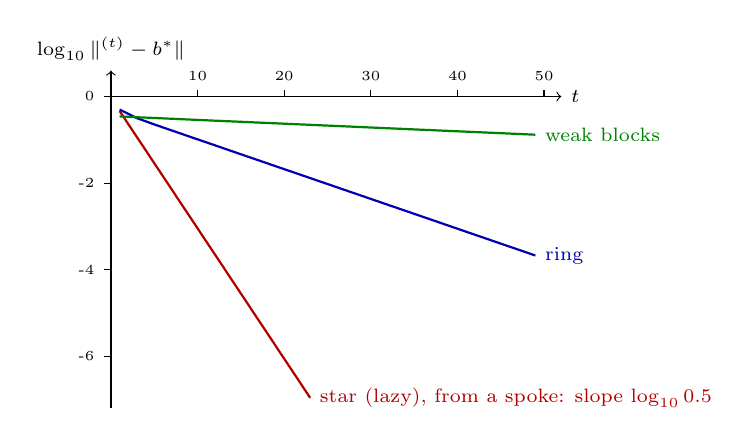
\begin{tikzpicture}[x=0.11cm, y=0.55cm]
\draw[->] (0,0) -- (52,0) node[right, font=\scriptsize] {$t$};
\draw[->] (0,-7.2) -- (0,0.6) node[above, font=\scriptsize] {$\log_{10}\|\bb^{(t)} - b^*\ones\|$};
\foreach \yy in {0,-2,-4,-6} \draw (0,\yy) -- (-0.8,\yy) node[left, font=\tiny] {\yy};
\foreach \xx in {10,20,30,40,50} \draw (\xx,0) -- (\xx,0.15) node[above, font=\tiny] {\xx};
\draw[red!70!black, thick] plot coordinates {(1,-0.335) (3,-0.937) (5,-1.539) (7,-2.141) (9,-2.743) (11,-3.345) (13,-3.947) (15,-4.549) (17,-5.151) (19,-5.753) (21,-6.355) (23,-6.957)};
\node[red!70!black, font=\scriptsize, right] at (23,-6.957) {star (lazy), from a spoke: slope $\log_{10}0.5$};
\draw[blue!70!black, thick] plot coordinates {(1,-0.301) (3,-0.499) (5,-0.644) (7,-0.782) (9,-0.920) (11,-1.057) (13,-1.195) (15,-1.333) (17,-1.470) (19,-1.608) (21,-1.745) (23,-1.883) (25,-2.020) (27,-2.158) (29,-2.295) (31,-2.433) (33,-2.570) (35,-2.708) (37,-2.845) (39,-2.983) (41,-3.121) (43,-3.258) (45,-3.396) (47,-3.533) (49,-3.671)};
\node[blue!70!black, font=\scriptsize, right] at (49,-3.671) {ring};
\draw[green!50!black, thick] plot coordinates {(1,-0.460) (3,-0.478) (5,-0.495) (7,-0.513) (9,-0.531) (11,-0.548) (13,-0.566) (15,-0.583) (17,-0.601) (19,-0.618) (21,-0.636) (23,-0.653) (25,-0.671) (27,-0.688) (29,-0.706) (31,-0.724) (33,-0.741) (35,-0.759) (37,-0.776) (39,-0.794) (41,-0.811) (43,-0.829) (45,-0.846) (47,-0.864) (49,-0.881)};
\node[green!50!black, font=\scriptsize, right] at (49,-0.881) {weak blocks};
\end{tikzpicture}
\end{center}

\solpart{c} On a log scale each curve becomes a straight line of slope $\log|\lambda_2|$. For the ring, the ratio $d_{t+1}/d_t$ is $0.7706$ at $t = 1$ (faster modes are still present), $0.8522$ at $t = 5$, and $0.8536$ from $t = 20$ on. A least-squares fit of $\ln d_t$ on $t$ over $t = 11, \ldots, 50$ gives $e^{\text{slope}} = 0.8536 = |\lambda_2|$. For the weak blocks the ratio is $0.98$ at every $t$, because $\mathbf{e}_1 - b^*\ones$ excites only the eigenvalues $0.98$ and $0$: the fitted rate is $0.9800$, and the half-life is $\ln 2/(-\ln 0.98) = 34.3$ rounds. For the star from a spoke the fitted rate over $t = 11, \ldots, 30$ is $0.5000$.

The reason is the proof of Proposition~\ref{ch08:prop:rate}. $\bb^{(t)} - b^*\ones = (W - \ones\boldsymbol{\pi}')^t(\bb^{(0)} - b^*\ones)$, and $W - \ones\boldsymbol{\pi}'$ has spectral radius $|\lambda_2|$. All four matrices are symmetric or reversible and so diagonalizable, so $\|\bb^{(t)} - b^*\ones\| \le C|\lambda_2|^t$ with equality in the limit whenever the initial deviation has a component on the $\lambda_2$ eigenspace. \emph{Common mistake:} expecting every starting vector to converge at rate $|\lambda_2|$. The rate is an upper bound; the hub start of the star shows that a deviation orthogonal to the slow modes converges faster.

%% ---------------------------------------------------------------------
\exercisesolution{6.4}{Bonacich with negative $\beta$}

\solpart{a} The matrix is symmetric with all row and column sums equal to one, so $\mathbf{d}^{\text{in}} = W'\ones = \ones$. Then $W'\ones = \ones$ gives $(I - \beta W')\ones = (1-\beta)\ones$, hence
\[
\mathbf{c}^{\text{Bon}}(\beta) = (I-\beta W')^{-1}\ones = \frac{1}{1-\beta}\ones,
\]
so $\mathbf{c}^{\text{Bon}}(0.3) = 1.4286\,\ones$ and $\mathbf{c}^{\text{Bon}}(-0.3) = 0.7692\,\ones$.
The inverse exists because the spectrum of $W$ is $\{1, -1, 0, 0\}$ and $|\beta| < 1$.

\solpart{b} \emph{As posed, the question has no non-trivial answer.} In this network every agent has the same centrality for every $\beta$. The graph is the complete bipartite graph $K_{2,2}$ with equal weights, and it is vertex-transitive: any agent can be mapped to any other by a permutation $P$ with $PWP' = W$, and Bonacich centrality is invariant under such permutations. Negative $\beta$ changes the level (from $1.4286$ to $0.7692$) but cannot separate agents who are structurally identical.

To see what negative $\beta$ does, break the symmetry. Buyer~1 trades only with seller~3, buyer~2 with sellers~3 and~4, and seller~4 only with buyer~2. Each row is uniform over the agent's partners, so $W$ has rows $(0,0,1,0)$, $(0,0,\frac12,\frac12)$, $(\frac12,\frac12,0,0)$, $(0,1,0,0)$ and in-degrees $(0.5, 1.5, 1.5, 0.5)$. Then
\begin{align*}
\mathbf{c}^{\text{Bon}}(0.3) &= (0.8075,\ 2.0497,\ 2.0497,\ 0.8075),\\
\mathbf{c}^{\text{Bon}}(-0.3) &= (0.3167,\ 1.2217,\ 1.2217,\ 0.3167).
\end{align*}
The two well-connected agents (2 and~3) lead in both cases, but their lead widens under bargaining: $c_2/c_1 = 2.54$ at $\beta = 0.3$ and $3.86$ at $\beta = -0.3$. With $\beta < 0$ the series $\mathbf{c} = \sum_k \beta^k (W')^{k}\mathbf{d}^{\text{in}}$ subtracts the centrality of your partners at odd path lengths. Agents~2 and~3 are partnered with agents (1 and~4) who have a single partner each, hence no outside option. That weakness is a source of bargaining strength for 2 and~3. This is Bonacich's reading of $\beta < 0$, and in the symmetric network of the exercise it has nothing to act on.

\solpart{c} \emph{Eigenvector.} $W$ is doubly stochastic, so by Proposition~\ref{ch06:prop:equal_power} $\boldsymbol{\pi} = (\frac14, \frac14, \frac14, \frac14)$. This agrees with the result the exercise attributes to \citet{manea2011bargaining}: equal bargaining power in a symmetric bipartite network. The agreement is a consequence of symmetry, not of a general correspondence: Assumption~7.A is a modelling postulate, and strategic bargaining payoffs are not eigenvector centralities in general.

\emph{Gap.} $W = \frac12\begin{pmatrix} 0 & J \\ J & 0\end{pmatrix}$ with $J = \ones_2\ones_2'$. Its eigenvalues are $1$ (eigenvector $\ones$), $-1$ (eigenvector $(1,1,-1,-1)'$) and $0, 0$. So $|\lambda_2| = 1$ and $\Gap = 0$. The value is zero because the network is bipartite, i.e.\ periodic with period~2: beliefs or influence alternate between the two sides, $W^t$ does not converge, and $(1,1,-1,-1)'$ flips sign every period. It does \emph{not} reflect fragmentation: the network is irreducible and the two sides are as connected as they can be. The lazy version $\frac12(I + W)$ has $\Gap = 0.5$ and the same $\boldsymbol{\pi}$. \emph{Common mistake:} reading $\Gap = 0$ here as ``disconnected'' or ``unequal''. It is neither.

%% ---------------------------------------------------------------------
\exercisesolution{6.5}{Power iteration by hand}

\solpart{a} $W' = \begin{pmatrix} 0.6 & 0.2 \\ 0.4 & 0.8\end{pmatrix}$. Starting from $\mathbf{v}^{(0)} = (1,1)'$:
\begin{center}
\begin{tabular}{cccc}
\toprule
$t$ & $W'\mathbf{v}^{(t-1)}$ & $\mathbf{v}^{(t)}$ (normalized) & $\max_i|v_i^{(t)} - \pi_i|$ \\
\midrule
1 & $(0.8,\ 1.2)$ & $(0.4,\ 0.6)$ & 0.06667 \\
2 & $(0.36,\ 0.64)$ & $(0.36,\ 0.64)$ & 0.02667 \\
3 & $(0.344,\ 0.656)$ & $(0.344,\ 0.656)$ & 0.01067 \\
4 & $(0.3376,\ 0.6624)$ & $(0.3376,\ 0.6624)$ & 0.00427 \\
5 & $(0.33504,\ 0.66496)$ & $(0.33504,\ 0.66496)$ & 0.00171 \\
\bottomrule
\end{tabular}
\end{center}
For instance, $t = 2$: $0.6(0.4) + 0.2(0.6) = 0.36$ and $0.4(0.4) + 0.8(0.6) = 0.64$. After the first step no normalization is needed: $\ones'W'\mathbf{v} = (W\ones)'\mathbf{v} = \ones'\mathbf{v}$, so $W'$ preserves the sum of a vector. The initial $\mathbf{v}^{(0)} = (1,1)'$ sums to $2$, and only that first normalization matters.

\solpart{b} The question depends on what ``converged to two decimal places'' means. The error first falls below $0.005$ at $t = 4$. The rounded iterate first equals the rounded limit $(0.33, 0.67)$ only at $t = 6$ ($\mathbf{v}^{(6)} = (0.334, 0.666)$). The iterates at $t = 3, 4, 5$ round to $(0.34, 0.66)$, because $\mathbf{v}^{(5)} = (0.33504, \ldots)$ is still just above the rounding boundary $0.335$. The error criterion is the right one; rounding agreement depends on how close the limit lies to a rounding boundary.

\solpart{c} $\boldsymbol{\pi}'W = \boldsymbol{\pi}'$ gives, from the first column, $0.6\pi_1 + 0.2\pi_2 = \pi_1$, i.e.\ $0.4\pi_1 = 0.2\pi_2$, so $\pi_2 = 2\pi_1$. With $\pi_1 + \pi_2 = 1$, $\boldsymbol{\pi} = (\frac13, \frac23)$. (The second column gives the same equation, as it must, since $W - I$ is singular.)

\solpart{d} The iterates approach $(\frac13, \frac23)$ monotonically from above in the first coordinate. The spectrum is $\{1, \tr W - 1\} = \{1, 0.4\}$, so $\Gap = 0.6$. The error ratios are exactly $0.4$ at every step: $0.02667/0.06667 = 0.01067/0.02667 = \cdots = 0.4 = |\lambda_2|$. In two dimensions this is exact, not asymptotic. Write $\mathbf{v}^{(t)} = \boldsymbol{\pi} + c_t\mathbf{u}$ with $\mathbf{u} = (1,-1)'$, a left eigenvector of $W$ for $0.4$ ($\mathbf{u}'W = (0.4, -0.4)$). Then $W'(\boldsymbol{\pi} + c\mathbf{u}) = \boldsymbol{\pi} + 0.4c\,\mathbf{u}$, and the sum stays $1$, so $c_{t} = 0.4^t c_0$. Each additional correct decimal costs $\ln 10/\ln(1/0.4) = 2.5$ iterations (Appendix~6A).

%% ---------------------------------------------------------------------
\exercisesolution{6.6}{Structural power vs.\ formal power}

\emph{A matrix} (agents ordered President, General, Businesswoman, Farmer; row $i$ is whom $i$ depends on):
\[
W = \begin{pmatrix}
0.30 & 0.20 & 0.20 & 0.30 \\
0.30 & 0.30 & 0.10 & 0.30 \\
0.10 & 0.10 & 0.40 & 0.40 \\
0.05 & 0.05 & 0.20 & 0.70
\end{pmatrix}. \illustrative
\]
\emph{Reading.} The President depends on the army ($0.2$), on business tax revenue ($0.2$) and on food for the cities and the palace ($0.3$). The General depends on the President's orders and budget ($0.3$), on his own corps ($0.3$) and on food rations ($0.3$). The Businesswoman's agro-processing and retail depend on farm output ($0.4$). The Farmer depends mostly on her own land and family labor ($0.7$), sells through the Businesswoman ($0.2$), and needs little from the state ($0.05$ each). Every row sums to one and every entry is positive, so $W$ is primitive.

\emph{Result.} $\boldsymbol{\pi} = (0.1178,\ 0.1060,\ 0.2367,\ 0.5395)$, $\Neff = 2.687$, $\Gap = 0.576$. The Farmer has the highest eigenvector centrality, more than four times the President's.

\emph{Verification.} The balance equation~\eqref{ch06:eq:perron_component} for the Farmer is
\[
\textstyle\sum_j\pi_jW_{j4} = 0.30(0.1178) + 0.30(0.1060) + 0.40(0.2367) + 0.70(0.5395) = 0.5395 .
\] Her column sum is $1.7$, the largest; but the ranking is not just in-degree. The Businesswoman (column sum $0.9$) ranks above the President ($0.75$) because the powerful Farmer places $0.2$ on her: indirect dependence (``directly or indirectly'') at work.

\emph{How robust is it?} If the President, General and Businesswoman each cut their food weight to $f$ (adding the difference to their own diagonal), the Farmer stays on top at $f = 0.30$ ($\pi_4 = 0.500$) and at $f = 0.20$ ($\pi_4 = 0.400$). At $f = 0.10$ she falls to $0.250$, behind the Businesswoman ($0.364$). Structural power from food dependence requires that the dependence be large \emph{relative} to the other links in each row, not merely present.

\emph{Interpretation.} Formal rank is a property of an organizational chart. Structural power is a property of the dependence matrix (Section~\ref{ch06:sec:practice}). It is the Perron weight that enters bargaining in Chapter~7 (by Assumption~7.A). \emph{Common mistakes:} (i) writing the Farmer's dependence on the others into her \emph{row} and expecting that to make her powerful. Power comes from the \emph{column}, from being depended upon (Proposition~\ref{ch06:prop:monotone}). (ii) Forgetting to make rows sum to one, which breaks the reading of $\boldsymbol{\pi}$ as power (Remark after Proposition~\ref{ch06:prop:equal_power}).

%% ---------------------------------------------------------------------
\exercisesolution{6.7}{Power in a stylized dual economy}

\solpart{a} Example~\ref{ch03:ex:bolivia} has $A_{\text{dual}} = \begin{pmatrix}0.15 & 0.03\\0.02 & 0.20\end{pmatrix}$ (rows Modern, Traditional), with row sums $(0.18, 0.22)$. Following the convention $W^P = D^{-1}A$ (Chapter~1, Section~\ref{ch01:sec:conventions}),
\[
W^P = \begin{pmatrix} 0.15/0.18 & 0.03/0.18 \\ 0.02/0.22 & 0.20/0.22\end{pmatrix} = \begin{pmatrix} 0.8333 & 0.1667 \\ 0.0909 & 0.9091\end{pmatrix}.
\]
This is a two-block matrix with leakages $\varepsilon_M = 0.1667$ and $\varepsilon_T = 0.0909$, so by Proposition~\ref{ch06:prop:block_power}, exactly,
\[
\pi_M = \frac{\varepsilon_T}{\varepsilon_M + \varepsilon_T} = \frac{0.0909}{0.2576} = 0.3529, \qquad \pi_T = 0.6471,
\]
with $\Gap = \varepsilon_M + \varepsilon_T = 0.2576$ and $\Neff = 1.841$.
Check: $0.3529 \times 0.8333 + 0.6471 \times 0.0909 = 0.3529$. \emph{The Traditional sector has the most structural power.} The answer surprises many students, but it follows from the definition. In $W^P$, being powerful means that others spend a large share of their input costs on you. The Modern sector spends $16.7\%$ of its (domestic intermediate) input costs on traditional inputs, while the Traditional sector spends only $9.1\%$ on modern inputs. Note that the absolute coefficients ($0.03$ vs $0.02$) and the input-cost shares point the same way here. The reading of $\pi$ in force is the production reading of \nolinkurl{docs/conventions.md}, \S2: $\pi$ is the $\gamma \to 1$ limit of the normalized influence vector, \emph{not} bargaining power, unless Assumption~7.A is adopted.

\solpart{b} No. $\boldsymbol{\pi}$ is a function of $W^P$ alone, and $W^P = D^{-1}A$ depends only on the technical coefficients. A transfer changes incomes and endowments $\boldsymbol{\omega}$, but not the recipe of either sector. So, holding $A$ fixed, $\boldsymbol{\pi}$ is unchanged (Section~\ref{ch06:sec:practice}, ``Power vs.\ Wealth''). The transfer would move $\boldsymbol{\pi}$ only if it changed $A$, for instance by changing what the traditional sector buys. That is an indirect, behavioral channel, which a fixed-$W$ model rules out by construction.

\solpart{c} With $a_{TM} = 0.15$, the Traditional row of $A$ becomes $(0.15, 0.20)$, with sum $0.35$:
\[
W^P_{\text{new}} = \begin{pmatrix} 0.8333 & 0.1667 \\ 0.4286 & 0.5714\end{pmatrix}, \qquad \boldsymbol{\pi}_{\text{new}} = (0.7200,\ 0.2800),
\]
with $\Gap = 0.5952$ and $\Neff = 1.676$.
\emph{The Traditional sector's power falls}, from $0.6471$ to $0.2800$ ($-0.3671$). The plant makes the Traditional sector depend on the Modern sector: weight in the Traditional row moves from $T$ to $M$. By Proposition~\ref{ch06:prop:monotone} (with $j = T$, $i = M$, $k = T$) that can only raise $\pi_M$. Integration rises: $\Gap$ goes from $0.258$ to $0.595$, as the bound $\Gap \le \varepsilon_M + \varepsilon_T$ of Proposition~\ref{ch06:prop:block_power} allows. Concentration of power also rises ($\Neff$ falls from $1.841$ to $1.676$), now in favor of the Modern sector.

The output side moves the other way, and it must be computed from $A$, not from $W^P$. The Leontief inverse $(I - A')^{-1}$ has column sums (output multipliers) $(1.2217, 1.2805)$ before and $(1.2287, 1.4804)$ after: a unit of traditional final demand now generates $0.2221$ units of modern output instead of $0.0294$. By contrast, a link in the other direction, $a_{MT}$ from $0.03$ to $0.15$ (the modern sector buying more from traditional suppliers), gives $\boldsymbol{\pi} = (0.1538, 0.8462)$: it raises the Traditional sector's power.

\solpart{d} Only the plant changes the power structure: it changes $A$, hence $W^P$, hence $\boldsymbol{\pi}$. The transfer leaves $\boldsymbol{\pi}$ unchanged. But the plant, as specified, changes it \emph{against} the Traditional sector, because buying from someone confers power on the seller, not the buyer. A structural policy meant to raise the traditional sector's Perron weight must make \emph{others} depend on it: purchases by the modern sector, by government procurement, or by processing plants that use traditional output as an input. \emph{Common mistake:} assuming that any new cross-block link ``integrates'' and therefore ``empowers'' the periphery. The plant does raise $\Gap$ and the multipliers, but it lowers $\pi_T$. Integration and the distribution of power are separate coordinates (Proposition~\ref{ch06:prop:gap-power-independent}).

\solpart{e} \emph{Data: real results.}
\begin{itemize}
\item \emph{Dataset.} INE Bolivia, \textit{Cuadros de Oferta y Utilizaci\'on}, base 2017, year 2019, current prices (\citealp{ine2026sut}). The table was converted in \texttt{data/compute/compute\_bolivia\_io.py} to a domestic industry-by-industry flow matrix $Z$ at basic prices (import proportionality, product-sales-structure model; \texttt{data/README.md}~\S2), aggregated to the book's 12 sectors (\texttt{book12}). File: \nolinkurl{data/processed/bolivia_Z/Z_2017_2019_book12.csv}; retrieved 2026-11-05. Domestic services has no intermediate flows and is dropped, leaving 11 sectors. (INE's older \textit{Matriz Insumo-Producto}, base 1990, ends in 2014; the base-2017 tables are the current ones.)
\item \emph{Check.} The 11-sector $W^P[s,s'] = Z[s',s]/\sum_k Z[k,s]$ (input-cost shares, rows = buyers) reproduces the values quoted in the exercise: $\Gap = 0.4674$ and $\Neff = 6.4795$ of 11 (Chapter~3, Section~\ref{ch03:sec:heterogeneity}). The largest Perron weights are other services (0.270), financial services (0.162) and manufacturing (0.159); hydrocarbons has $0.039$.
\item \emph{Aggregation.} Choose a partition into Modern and Traditional, let $M$ be the $11\times 2$ membership matrix, set $Z_2 = M'ZM$ (sum the flows), and form $W^P_2$ from $Z_2$ in the same way. The 12-sector classification does not separate large from small firms, so no partition matches Example~\ref{ch03:ex:bolivia} exactly; we report three.
\end{itemize}
\begin{center}
\footnotesize
\setlength{\tabcolsep}{4pt}
\begin{tabular}{lcccccc}
\toprule
Modern block & $\varepsilon_M$ & $\varepsilon_T$ & $\pi_M$ & $\Neff$ (of 2) & $\lambda_2$ & $\Gap$ \\
\midrule
Hydrocarbons, Mining, Financial & 0.7620 & 0.1904 & 0.2000 & 1.471 & 0.0476 & 0.952 \\
\quad + Manufacturing & 0.5435 & 0.4283 & 0.4407 & 1.972 & 0.0283 & 0.972 \\
\quad + Publ.\ adm., Transport, Oth.\ serv. & 0.3222 & 0.7023 & 0.6855 & 1.758 & $-0.0246$ & 0.975 \\
\midrule
Stylized (Example~\ref{ch03:ex:bolivia}) & 0.1667 & 0.0909 & 0.3529 & 1.841 & 0.7424 & 0.258 \\
\bottomrule
\end{tabular}
\end{center}
Here $\varepsilon_M$ is the share of the modern block's domestic intermediate input costs spent on the traditional block, and vice versa. For a $2\times 2$ row-stochastic matrix $\lambda_2 = 1 - \varepsilon_M - \varepsilon_T$, so $\Gap = 1 - |1 - \varepsilon_M - \varepsilon_T|$.

\emph{Comparison and answer.} Every two-sector aggregation makes Bolivia look \emph{far more} integrated ($\Gap \approx 0.95$--$0.98$) than the 11-sector table ($0.467$), and far more than the stylized model ($0.258$). Two reasons:
\begin{enumerate}
\item \emph{The data do not have the stylized enclave's small cross-block shares.} In the narrow definition the extractive and financial block spends $76\%$ of its domestic input costs on the rest of the economy. The stylized model assumes $17\%$. On the integration coordinate, Bolivia's measured $W^P$ is not block-diagonal, as the Prebisch box of Section~\ref{ch06:sec:gap} reports.
\item \emph{Aggregation removes slow modes.} If a partition is exactly lumpable ($W M = M\bar W$), every eigenvalue of $\bar W$ is an eigenvalue of $W$ (if $\bar W\bar{\x} = \lambda\bar{\x}$ then $W(M\bar{\x}) = \lambda M\bar{\x}$), so $\Gap(\bar W) \ge \Gap(W)$. The slow mode $\lambda_2 = 0.533$ of the 11-sector matrix runs \emph{within} what the partitions lump together, and the two-block matrix cannot represent it.
\end{enumerate}
Power is a separate coordinate, and it depends on the partition: $\pi_M$ ranges from $0.20$ to $0.69$ as the modern block grows. Compare concentration as $\Neff/N$ (Chapter~6 conventions): $0.735$--$0.986$ for the two-block versions and $6.48/11 = 0.589$ at 11 sectors. Like $\Gap$, a single number from an arbitrary partition is not informative; only like-for-like comparisons are.

\emph{Common mistakes:} comparing $\Gap$ or $\Neff$ across aggregation levels or node sets; computing $W^P$ by normalizing the rows of the published table (those are \emph{sales} shares, rows = suppliers); and including imported inputs, which mixes the domestic structure with the import structure.

\end{document}
